\documentclass[tikz,border=3pt]{standalone}
\usepackage[utf8]{inputenc}
\usepackage[T1]{fontenc}
\usepackage{lmodern}
\renewcommand{\familydefault}{\sfdefault}
\usepackage{sansmath}\sansmath
\usepackage{chemfig}
\usepackage{pgfplots}\pgfplotsset{compat=1.18,/pgf/number format/use comma,/pgf/number format/1000 sep={.}}
\usetikzlibrary{arrows.meta,calc,positioning,decorations.pathmorphing,patterns}
% paleta del sitio
\definecolor{nar}{HTML}{E8680C}\definecolor{narc}{HTML}{FFB35C}\definecolor{hielo}{HTML}{FFF3E8}
\definecolor{tinta}{HTML}{1D1D1F}\definecolor{gris}{HTML}{6E6E73}\definecolor{lila}{HTML}{7C5CF0}
\definecolor{azul}{HTML}{2F6FD6}\definecolor{menta}{HTML}{17A673}\definecolor{coral}{HTML}{E8342A}
\begin{document}
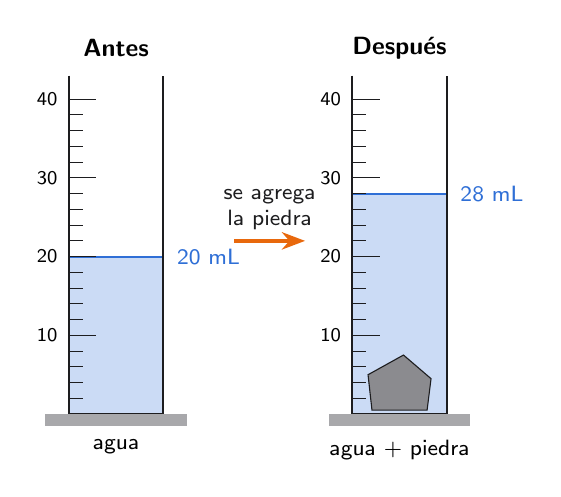
\begin{tikzpicture}[font=\small]
\fill[azul!25] (0,0) rectangle (1.2,2);
\draw[azul,thick] (0,2) -- (1.2,2);
\draw[tinta,thick] (0,4.3) -- (0,0) -- (1.2,0) -- (1.2,4.3);
\fill[gris!60] (-0.3,-0.15) rectangle (1.5,0);
\draw[tinta] (0,0.2) -- (0.18,0.2);
\draw[tinta] (0,0.4) -- (0.18,0.4);
\draw[tinta] (0,0.6) -- (0.18,0.6);
\draw[tinta] (0,0.8) -- (0.18,0.8);
\draw[tinta] (0,1) -- (0.35,1);
\node[anchor=east,font=\scriptsize] at (-0.02,1) {10};
\draw[tinta] (0,1.2) -- (0.18,1.2);
\draw[tinta] (0,1.4) -- (0.18,1.4);
\draw[tinta] (0,1.6) -- (0.18,1.6);
\draw[tinta] (0,1.8) -- (0.18,1.8);
\draw[tinta] (0,2) -- (0.35,2);
\node[anchor=east,font=\scriptsize] at (-0.02,2) {20};
\draw[tinta] (0,2.2) -- (0.18,2.2);
\draw[tinta] (0,2.4) -- (0.18,2.4);
\draw[tinta] (0,2.6) -- (0.18,2.6);
\draw[tinta] (0,2.8) -- (0.18,2.8);
\draw[tinta] (0,3) -- (0.35,3);
\node[anchor=east,font=\scriptsize] at (-0.02,3) {30};
\draw[tinta] (0,3.2) -- (0.18,3.2);
\draw[tinta] (0,3.4) -- (0.18,3.4);
\draw[tinta] (0,3.6) -- (0.18,3.6);
\draw[tinta] (0,3.8) -- (0.18,3.8);
\draw[tinta] (0,4) -- (0.35,4);
\node[anchor=east,font=\scriptsize] at (-0.02,4) {40};
\node[font=\small\bfseries] at (0.6,4.65) {Antes};
\node[anchor=west,font=\footnotesize,text=azul] at (1.25,2) {20 mL};
\fill[azul!25] (3.6,0) rectangle (4.8,2.8);
\draw[azul,thick] (3.6,2.8) -- (4.8,2.8);
\fill[gris!80,draw=tinta] (3.85,0.05) -- (4.55,0.05) -- (4.6,0.45) -- (4.25,0.75) -- (3.8,0.5) -- cycle;
\draw[tinta,thick] (3.6,4.3) -- (3.6,0) -- (4.8,0) -- (4.8,4.3);
\fill[gris!60] (3.3,-0.15) rectangle (5.1,0);
\draw[tinta] (3.6,0.2) -- (3.78,0.2);
\draw[tinta] (3.6,0.4) -- (3.78,0.4);
\draw[tinta] (3.6,0.6) -- (3.78,0.6);
\draw[tinta] (3.6,0.8) -- (3.78,0.8);
\draw[tinta] (3.6,1) -- (3.95,1);
\node[anchor=east,font=\scriptsize] at (3.58,1) {10};
\draw[tinta] (3.6,1.2) -- (3.78,1.2);
\draw[tinta] (3.6,1.4) -- (3.78,1.4);
\draw[tinta] (3.6,1.6) -- (3.78,1.6);
\draw[tinta] (3.6,1.8) -- (3.78,1.8);
\draw[tinta] (3.6,2) -- (3.95,2);
\node[anchor=east,font=\scriptsize] at (3.58,2) {20};
\draw[tinta] (3.6,2.2) -- (3.78,2.2);
\draw[tinta] (3.6,2.4) -- (3.78,2.4);
\draw[tinta] (3.6,2.6) -- (3.78,2.6);
\draw[tinta] (3.6,2.8) -- (3.78,2.8);
\draw[tinta] (3.6,3) -- (3.95,3);
\node[anchor=east,font=\scriptsize] at (3.58,3) {30};
\draw[tinta] (3.6,3.2) -- (3.78,3.2);
\draw[tinta] (3.6,3.4) -- (3.78,3.4);
\draw[tinta] (3.6,3.6) -- (3.78,3.6);
\draw[tinta] (3.6,3.8) -- (3.78,3.8);
\draw[tinta] (3.6,4) -- (3.95,4);
\node[anchor=east,font=\scriptsize] at (3.58,4) {40};
\node[font=\small\bfseries] at (4.2,4.65) {Después};
\node[anchor=west,font=\footnotesize,text=azul] at (4.85,2.8) {28 mL};
\node[anchor=north,font=\footnotesize] at (0.6,-0.2) {agua};
\node[anchor=north,font=\footnotesize,align=center] at (4.2,-0.2) {agua + piedra};
\draw[-{Stealth},very thick,nar] (2.1,2.2) -- (3.0,2.2) node[midway,above,font=\footnotesize,text=tinta,align=center] {se agrega\\la piedra};

\end{tikzpicture}
\end{document}
